%sec1-6
\begin{center}
    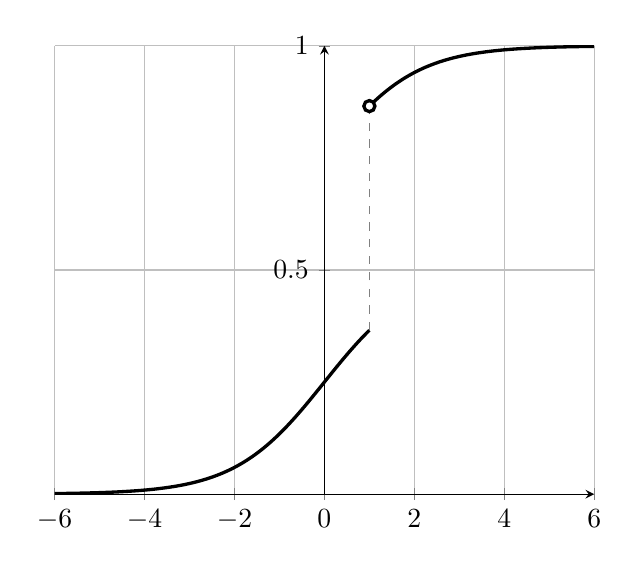
\begin{tikzpicture}[
        declare function={
            sigma(\x)=1 / (1 + exp(-\x));
            F(\x) = .5 * sigma(\x);
        }]
        \begin{axis}[
            grid=major,     
            xmin=-6, xmax=6,
            ymin=0, ymax=1,
            ytick={0,.5,1},
            axis x line=bottom,
            axis y line=middle,
            samples=100,
            legend style={at={(1,0.9)}}     
        ]
        \addplot[very thick,black,mark=none, domain=-6:1]   {F(x)};
        \addplot[very thick,black,mark=*,mark options={fill=white},domain=1:6, mark repeat=1000]    {F(x)+0.5};
        \draw [dashed,black!50] (1,{F(1)}) -- (1,{F(1)+0.5});        
        \end{axis}
    \end{tikzpicture}
\end{center}